% \documentclass[11pt,letterpaper]{article}
% %\usepackage[ruled,vlined,commentsnumbered,titlenotnumbered]{algorithm2e}

\documentclass[10pt]{article}

% Sort alphabetically by package name.
\usepackage[a4paper, margin=2cm]{geometry}
\usepackage{graphicx}
\usepackage{times}

\usepackage{url}


\usepackage[subtle,mathspacing=normal]{savetrees}
%\setlength{\oddsidemargin}{0pt}
%\setlength{\evensidemargin}{0pt}
%\setlength{\textwidth}{6.5in}
\setlength{\textheight}{8.7in}



%\setlength{\oddsidemargin}{0pt}
%\setlength{\evensidemargin}{0pt}
%\setlength{\textwidth}{6.5in}
%\setlength{\topmargin}{0in}
%\setlength{\textheight}{9in}
%\usepackage{refcheck}
%\usepackage{pslatex} % use times roman
\usepackage{amsmath}
\usepackage{algorithm}
\usepackage[noend]{algpseudocode}
\usepackage{amssymb}
\usepackage{amsthm}
\usepackage{color}
\usepackage{array}
\usepackage{xy}
\usepackage{setspace}
\usepackage{varwidth}% http://ctan.org/pkg/varwidth
\usepackage{multicol}
\usepackage{algorithm}
\usepackage{hyperref}
%%\doublespacing
%\usepackage{natbib}
%% \usepackage{cite}
%% \usepackage[margin=1in,letterpaper]{geometry}
%% \setlength{\topmargin}{0 in}
%% \setlength{\textheight}{9 in}
\usepackage{todonotes}

%% \documentclass[12pt,letterpaper]{amsart}
%% \setlength{\oddsidemargin}{0pt}
%% \setlength{\evensidemargin}{0pt}
%% \setlength{\textwidth}{6.5in}
%%\setlength{\topmargin}{1in}
%% \setlength{\textheight}{9in}
%% %\usepackage{refcheck}
%% \usepackage{pslatex} % use times roman
%% \usepackage{amsmath}
%% \usepackage{amssymb}
%% \usepackage{amsthm}
%% \usepackage{color}
%% \usepackage{array}
%% \usepackage{xy}
%% \usepackage{setspace}

%\usepackage[left=1.5in,right=1.5in, top=1.5in,bottom=1.5in,]{geometry}

\newcommand{\NN}{\mathbb{N}} \newcommand{\ZZ}{\mathbb{Z}}
\newcommand{\range}{\text{ran}}
\newcommand{\poly}{\operatorname{poly}}
\newcommand{\domain}{\text{dom}} \newcommand{\im}{\text{im}}
\newcommand{\sign}{\operatorname{sign}} \newcommand{\si}{\mathbf{S}}
\newcommand{\OR}{\vee} \newcommand{\E}{\mathbb{E}}
\newcommand{\AND}{\wedge} \newcommand{\PP}{\mathcal{P}}
\newcommand{\edit}{\operatorname{ed}}
\newcommand{\dtw}{\operatornamewithlimits{DTW}}
\newcommand{\ed}{\operatorname{ed}}
\newcommand{\ham}{\operatorname{Ham}}
\newcommand{\alg}{\operatorname{ALG}}
\newcommand{\slide}{\operatorname{slide}}
\newcommand{\dist}{\Delta_{\ell_1}}
\newcommand{\argmin}{\operatornamewithlimits{argmin}}
\newcommand{\subproblem}{\operatornamewithlimits{endToMiddle}}
\newcommand{\xrun}{r_x} \newcommand{\yrun}{r_y}
\newcommand{\yrunlength}{l_y} \newcommand{\yprevrunlength}{p_y}
\newcommand{\xrunlength}{l_x} \newcommand{\yoffset}{o_y}
\newcommand{\xoffset}{o_x}
\newcommand{\yrunoffset}{o_x}
\newcommand{\xrunoffset}{o_y}
\newcommand{\tipToMiddle}{\operatorname{SP}}
\newcommand{\rundiff}{d}


%----------------MACROS---------------%
%% \newtheoremstyle{slanted}% <name>
%% {3pt}% <Space above>
%% {3pt}% <Space below>
%% {\slshape}% <Body font>
%% {}% <Indent amount>
%% {\bfseries}% <Theorem head font>
%% {.}% <Punctuation after theorem head>
%% {.5em}% <Space after theorem heading>
%% {}% <Theorem head spec (can be left empty, meaning `normal')>


\newtheorem{thm}{Theorem}[section]
\newtheorem{lem}[thm]{Lemma}
\newtheorem{prop}[thm]{Proposition}
\newtheorem{clm}[thm]{Claim}
\newtheorem{cor}[thm]{Corollary}
\newtheorem{conj}[thm]{Conjecture}
\theoremstyle{remark}
\newtheorem{rem}[thm]{Remark}
\newtheorem{ex}[thm]{Example}

\newtheorem{theorem}{Theorem}[section]
\newtheorem{definition}[thm]{Definition}
\newtheorem{lemma}[thm]{Lemma}
\newtheorem{proposition}[thm]{Proposition}
\newtheorem{claim}[thm]{Claim}
\newtheorem{corollary}[thm]{Corollary}
\newtheorem{conjecture}[thm]{Conjecture}
\theoremstyle{remark}
\newtheorem{remark}[thm]{Remark}
\newtheorem{example}[thm]{Example}
\newtheorem{observation}[thm]{Observation}
\newcommand{\defn}[1]{\textbf{\emph{#1}}}
\renewcommand{\paragraph}[1]{\vspace{.2 cm} \noindent \textbf{#1}}
\newcommand{\wt}{\text{wt}}
\newcommand{\aug}{\text{Aug}}
\usepackage{authblk}


\newcommand{\figref}[1]{Figure~\ref{fig:#1}}
\newcommand{\figlabel}[1]{\label{fig:#1}}

\title{Practical Graveyard Hashing}
\author{Michael A. Bender \and
        Bradley C. Kuszmaul \and
        William Kuszmaul}
\begin{document}
\maketitle

What are the requirements for a practical C++ hash table?
\begin{itemize}
\item Near-compatability with the C++ standard library hash table
  containers (\texttt{std::unordered\_set} and
  \texttt{std::unordered\_map}).  These are templated (parameterized)
  tables in which the user can specify a key, a hash function, and an
  equality function.  The tables support heterogeneous lookup (which
  allows you to construct something that can be hashed or compared to
  a key without actually constructing a key).  The stability
  properties can weaker.
    
\item Slightly weaker stability requirements than the C++ standard library containers.  This is about what happens to pointers to objects in the table.  In the standard library containers, you can get the pointer to an object that is stored in the table. Stability is the issue of how long that pointer remains valid.  For example, in the standard library
  \begin{itemize}
    \item If you destroy the table, any pointers into the table become invalid.
    \item There is also an \textit{iterator} that lets you step
      through all the values in a table.  An iterator value may
      reference a value in the table.  If you destroy the table, any
      existing iterators become invalid.
    \item If you erase an element from the table, then iterators and
      pointers that currently reference that element become invalid.
      Other iterators and pointers remain valid.
    \item If the table is rehashed (e.g., because it got too big),
      then all iterators become invalid, but all pointers remain valid.
   \end{itemize}

  In order to accommodate open-addressed hash tables, both Google and
  Facebook have adopted the modification to those rules:
  \begin{itemize}
  \item  If a table is rehashed, then its pointers also become invalid.
  \end{itemize}

   For example, the following code can result in undefined behavior
   (which means that your computer may crash or that all your files
   could be erased, among other things).
\begin{verbatim}
   // Define a set of integers
   flat_hash_map<int, int> table;
   
   table[42] += table[43];
\end{verbatim}
This can crash using the Google/Facebook tables, since
\texttt{table[42]} implicitly inserts a \texttt{42} into the table if
it isn't already there, and then `table[43]` implicitl inserts a
\texttt{43} into the table if isn't there.  (The order in which those
two inserts is performed is implementation-defined.  GCC does it in
one order, whereas Clang does it in the other).  The problem is that
the second insert may cause the table to rehash, invalidating the
pointer returned by the first insert, so when the \texttt{+=} operator
runs, it may be passed an invalid pointer.

  In order to prevent a table from being rehashed, people use the
  \texttt{reserve(n)} function, which guarantees that the hash table
  can hold $n$ values without rehashing (by rehashing the table
  immediately if necessary).  For example, if you write
\begin{verbatim}
  table.reserve(table.size() + 2);
  table[42] += table[43];
\end{verbatim}
  then you know that the table can absorb two more insertions without
  rehashing, and hence you know that the table won't be rehashed even
  if both 42 and 43 end up being inserted

  Note: Erasing from the table doesn't give you any credit.  If you
  reserve (table.size()+2) then erase one element, and then insert
  three, your table may get rehashed on the third insert.  The
  guarantee is ``No rehash will occur during the next \texttt{n -
    table.size()} insertions.''

\item Performance (cache locality).  One of the points of using these
  tables is to reduce the number of cache misses.  A chained hash
  table would have many cache misses for a lookup, whereas these
  tables use open addressing to try to reduce the number of cache
  misses.

\item Memory parsimony: Chained hash tables also have to pay memory
  for the pointers in the linked lists.  These tables try to save that
  memory by using open addressing.  The Google hash table can run at
  up to 7/8 full.  Unfortunately, in practice the Google hash tables
  run more like at 55\% to 65\% full, since when it rehashes it
  doubles the table size (it uses power-of-two table sizes) and
  reduces the load to 7/16 full.  This ought to produce a table that
  runs at 62\% full (if Benford's rule applies, you expect the
  geometric mean of the low- and hi- load factor.  \cite{Benford38})  The calculations
  for the Facebook table are similar.

\item Not a requirement: Fine-grained parallelism.  Many authors data
  structures in the literature provide fine-grained lock-free
  parallelism, for example.  This is useless in a systems context,
  since there is no way to compose operations on that data structure
  with other operations to produce an atomic operation.  Real systems
  generally employ mutex locks, and require that the data structure be
  thread-compatible: that is, operations marked \texttt{const} may be
  called concurrently, and other operations need synchronization, such
  as a mutex, which is generally not part of the data structure.

\item Header-only: This isn't a requirement on the API, but an
  implementation that can be used as a set of headers is easier to
  integrate than an implementation that requirs building libraries and
  integrating them into a build system.  For example, the Facebook
  hash table uses CMake, and the Google table uses Bazel.  If you
  aren't already using the right build system, good luck.  A
  header-only library works by installing some header files to a
  directory and adding that directory to your compiler's search path.
\end{itemize}

Explain tombstones and graveyards.

Our table:
\begin{itemize}
\item Runs at 3/4 to 7/8 full (81\% on average if you believe in
  Benford's rule \cite{Benford38}).  In our benchmarks, we use about 30\% less memory
  than the Facebook or Google tables.
\item Performance is about the same as the Facebook or Google tables.
\item High-water memory is 33\% lower.
\item Deamortized inserts to reduce the tail latencies.  (By 6 orders
  of magnitude).
\item Graveyard tombstones.
\end{itemize}

Results?
\begin{itemize}
  \item Graveyard tombstones show value at very high load factors (TODO).  At
    lower load factors, the difference is less significant.  
  \item How many tombstones do you need?  The theory says to do something like this:
    \begin{itemize}
    \item Rehash the table when it's 92.5\% full down to 90\% full.
    \item Make 5\% of the rehashed table be evenly-spaced graveyard
      tombstones, the other 5\% empty slots occur whereever there are
      holes after the insertion from the rehash.
    \end{itemize}
    We probably don't need so many graveyard tombstones, partly since
    rehashing is so fast compared to insertions.  We found that X\%
    was enough.
\end{itemize}

Experiments to run:
\begin{itemize}
\item Determine how much impact graveyard tombstones make.  May need to measure it at high load factors.

  It looks like graveyard hashing slows things down at 9092.  Inserts shouldn't be worse, so what's going on?  Maybe the wrong number of tombstones.

  Should we measure a wide variety of tombstone-counts at various high loads?
\end{itemize}

One bubble-sort step: prove that it is pretty good.

Hover workload: It looks like for a 3/4 full table, after doing t.size() hovers, the unsuccessful search cost has gone up from 1.018 probes to 1.276 probes.
For a 90\% full table, the unsuccessful search cost quickly rises from 1.2 to 1.6 after 10\%, then 2.2 after another 10\%.
Conclusion:  You should rehash after doing N hovers if you would have rehashed after doing N inserts.

\section{The Algorithmics of Query-Optimized Graveyard Hashing}

\subsection{Background: Linear Probing, Ordered Linear Probing, and Graveyard Hashing}

\paragraph{Classical linear probing.} First introduced in 1954 \cite{??}, linear probing is one of the simplest possible hash table designs. Elements are stored in an array $A$ of some size $n$. To insert an item $u$, we examine slots $A[(h(u) + i) \mod n]$ for $i = 0, 1, 2, \ldots$ until we find a slot where the element can go. To query an element $u$,  we examine slots $A[(h(u) + i) \mod n]$ for $i = 0, 1, 2, \ldots$ until either we find $u$ or until we encounter an empty slot, in which case we can deduce that $u$ is not present. To delete an element $u$, we simply replace the element with a \defn{tombstone}.\footnote{There are also several other approaches that one can take to implement deletions \cite{...}. Tombstones allow for stability (which we want) and naturally lead to graveyard hashing (which we will describe in a moment).} Tombstones interact asymmetrically with insertions and queries: insertions treat tombstones as available slots that can be overwritten with new elements, and queries treat tombstones as occupied slots that must be skipped over. Finally, in order to avoid the over-accumulation of tombstones, one should occasionally rebuild the hash table and clear out all of the tombstones---if the hash table is filled to a load factor of $1 - 1/x$ full, then it suffices to perform such a rebuild once every $O(n/x)$ insertions. These rebuilds are typically also used as an opportunity to resize the hash table.

Linear probing has many of the features that one desires from a hash table. It exhibits excellent cache locality, as each operation accesses just one contiguous region of memory. It is naturally stable\todo{defined stable?} between rebuilds, making it a suitable choice for a library hash table. And it is extremely simple to implement.

However, linear probing also famously comes with a major drawback \cite{...}: as elements are placed into the hash table, they have a tendency to \emph{cluster} together into long runs. If the hash table is filled to a load factor of $1 - 1/x$, and then we look at a random position $p$ in the table, the expected distance from position $p$ to the next free slot ends up being $\Theta(x^2)$ (not the $\Theta(x)$ bound one might naturally expect!). This means that the expected time to perform an insertion is $\Theta(x^2)$, that the expected time to perform a negative query is $\Theta(x^2)$, and that the expected time to perform a positive query \emph{can be} $\Theta(x^2)$.\footnote{The time to query an element is the same as the time that was previously spent inserting it. If an element was inserted at a load factor of $1 - 1 /x$, then the expected time to query that element will be $O(x^2)$. So the expected time to query an element is actually \emph{a function} of the load factor at which the element was inserted.} 

This \defn{clustering effect} causes linear probing to scale poorly as the hash table fills to high load factors. This is widely cited as a central reason that researchers often turn to other hash table designs (e.g., quadratic probing \cite{...}, double hashing \cite{...}, cuckoo hashing \cite{...}) when designing library hash tables.

\paragraph{Salvaging queries with ordered linear probing.} In 1973, Amble and Knuth \cite{AmbleKn74} showed how to how to modify linear probing in order to improve query time to $O(x)$. 

Notice that, even in classical linear probing, not all positive queries are slow. If we fill a table from empty to $1 - 1/x$ full, then the vast majority of elements will have been inserted \emph{when the hash table was still relatively empty}. These elements $u$ are much quicker to query. In fact, if we define the \defn{offset} of an element $u$ to be the distance between where $u$ resides and its target position $h(u)$, then the \emph{average offset} across all the elements in the hash table will be $O(x)$. The problem is that these offsets are not evenly $O(x)$ across the board---elements that were inserted at load factor close to $1 - 1/x$ will have much higher offsets on average. 

To resolve this problem, Amble and Knuth propose that within each run of elements, the elements should be stored in \emph{sorted order by hash}. This naturally causes elements to have small offsets (regardless of when they are inserted!), and results in \emph{every} query having an expected running time of $O(x)$. In fact, even negative queries benefit, since they no longer have to find an empty slot in order to terminate---instead, they terminate as soon as they encounter any element $u'$ whose hash $h(u')$ is larger than the hash $h(u)$ of the element $u$ being queried.

This technique is known as \defn{ordered linear probing} (or, more popularly, as \defn{Robin Hood hashing} \cite{??}). Ordered linear probing eliminates the effects of clustering for queries. But it introduces two additional problems that have prevented it from becoming widely used in practice:
\begin{enumerate}
    \item \textbf{Instability: }To keep each run in sorted order, an insertion may have to rearrange multiple elements. This violates the stability property that many library hash tables require. 
    \todo{Thus, ordered-linear probing does not serve as general replacement for LP in library settings where stability is nonnegotiable. }
    \item \textbf{Hashing Overhead:} Both (negative) queries and insertions must compute the hash of every element $u'$ that they encounter. This can add substantial practical overhead.\todo{Michael feels that maybe we should write a bit more here. E.g., why isn't this just a small engineering tweak.}
\end{enumerate}

We will revisit both of these issues later on, when we design query-optimized graveyard hashing.

\paragraph{Salvaging insertions with graveyard hashing.} Recently, Bender, Kuszmaul, and Kuszmaul \cite{??} showed how to further modify linear probing in order to eliminate the asymptotic effects of clustering for \emph{all} operations, including insertions. 

A \defn{graveyard hash table} is an ordered linear-probing hash table with the following modification: each time that the hash table is rebuilt, \emph{artificial tombstones} are added into the hash table. These tombstones create holes within each run that future insertions can make use of (without going to the end of the run!). Just as for classical linear probing, the rebuilds are performed every $\Theta(n/x)$ insertions (say, $n/(4x)$), and the first thing that a rebuild does is remove any tombstones that are currently present. However, the rebuild now \emph{also} adds $\Theta(n/x)$ new artificial tombstones (say, $n/(2x)$) evenly spread across the hash table (one tombstone every $\Theta(x)$ positions). Critically, there should be enough artificial tombstones that if \emph{every} insertion (all $n/(4x)$) between now and the next rebuild window were to use an artificial tombstone, that would only use a constant fraction (in this case, half) of the artificial tombstones.

The artificial tombstones make it so that, at a load factor of $1- 1/x$, the expected amortized time per insertion is now $O(x)$ (not the $O(x^2)$ bound that clustering would give!). Additionally, since graveyard hashing still uses Amble and Knuth's ordering trick, queries are also $O(x)$ expected time. On the other hand, this means that graveyard hashing also still suffers from both of the Instability and Hashing Overhead problems discussed above.

\subsection{This Paper: Query-Optimized Graveyard Hashing}
\todo{Michael doesn't like name: polished, library-quality, .... what adjective should we use?}

This paper introduces query-optimized graveyard hashing, a new version of graveyard hashing that eliminates both the Instability and the Hashing Overhead problems described in the previous subsection. As we shall see in later subsections, this allows for us to implement a practical and theoretically sound library hash table that scales well to high load factors (without any of the classical clustering effects associated with linear probing!).

Before we describe query-optimized graveyard hashing, it is worth foreshadowing what makes it interesting. The artificial tombstones, which were introduced as a tool to speed up \emph{insertions}, will now play a critical role in ensuring fast \emph{queries} as well. Indeed, they are what will make it possible for us to overcome the issues traditionally associated with ordered linear probing (instability and hashing overhead) without compromising asymptotic query performance.

\paragraph{Query-Optimized Graveyard Hashing.}
To facilitate our discussion, we will think of the array as being partitioned into \defn{bins} of size $O(x)$. We say that an element $u$ \defn{hashes to a bin $B$} if $h(u) \in B$ (note that $u$ could hash to a bin $B$ but end up residing in a different bin). 

The first thing to know about query-optimized Graveyard hashing is that it is only \emph{partially}\todo{"partly" is probably better than "partially", since "partially ordered" has a meaning} ordered. Whenever a rebuild occurs, the elements are reordered to be in sorted order by hash. But insertions that occur between rebuilds do not worry about maintaining the ordering invariant. They can simply make use of whatever tombstones or free slot they first encounter. This partial ordering property is what (1) gives the hash table stability between rebuilds and (2) eliminates hashing overhead for insertions. (Note that it does not eliminate hashing overhead during rebuilds, but rebuilds have to rehash items anyway in order to insert/delete tombstones and handle resizing.)

The partial ordering property creates a problem for queries, however. Notably, a query for some element $u$ can no longer simply terminate as soon as it finds some element $u'$ satisfying $h(u') > h(u)$. (Also, we don't want the query to have to compute the hashes of the elements it encounters, but that's a separate issue.) 

To help queries run faster, we add a \defn{query counter}\todo{let's think carefully about this terminology.  BCK uses "search distance" in the code.  One problem is that "query counter" might make people think we are counting the number of queries.  This also isn't a counter since it isn't incremented. 
 It's \texttt{max}'d.  Perhaps call it a \textit{query bound}.} $q_B$ to each bin $B$. The query counter is guaranteed to be an upper bound on the maximum offset currently incurred by any element $u$ that hashes to bin $B$. Thus, if a query $u$ hashes to bin $B$, then the query can terminate as soon as it has traveled distance more than $q_B$ (as this indicates that $u$ is not in the hash table!). 

Query counters are updated as follows. Whenever a rebuild occurs, the query counter $q_B$ for each bin $B$ is recomputed from scratch. Then, between rebuilds, each insertion updates the query counter for the appropriate bin. That is, if the insertion inserts an element $u$ that hashes to bin $B$ and has offset $r$, then the counter $q_B$ becomes $\max(q_B, r)$. Deletions do not have to update query counters, since the query counter needs only to be an \emph{upper bound} (rather than an exact bound) on the maximum 
offset of any element hashing to the bin. 

Note that query counters would be useless for classical linear probing. Indeed, within each bin there is expected to be $1$ element that was inserted quite recently (say, after the most recent rebuild), and that element has expected offset $\Theta(x^2)$!\todo{Watch out for ! being read as "factorial"} This is where graveyard hashing comes to the rescue: the artificial tombstones left behind by graveyard hashing ensure that whenever an element is inserted, its expected offset is $O(x)$. The result (although this will require some effort to show) is that each query counter has expected value $O(x)$. This is what allows for us to implement both positive and negative queries in expected time $O(x)$ while only using partial ordering (and without the hashing overhead associated with full ordering).

The pseudocode for insertions/deletions/queries/rebuilds is given in Algorithm \ref{??}.

\paragraph{The analysis.}
In the rest of the section, we prove the following theorem:
\begin{theorem}
Consider a query-optimized graveyard hash table that is dynamically resized to have load factor $1 - \Theta(1/x)$ at all points in time. Then queries take expected time $O(x)$ and insertions/deletions take amortized expected time $O(x)$. 
\end{theorem}

... Analysis works with good families of hash functions...

... Corollary for external-memory hash tables...

... Corollary for vectorized version ...


\subsection{One More Algorithmic Contribution: Simple In-Place Resizing}



\subsection{...}





As we shall see, query counters allow for negative queries to complete in expected time $O(x)$ (without incurring hashing overhead!). 


add \emph{query counters} spaced every $O(x)$ positions. A 


\section{Experiment 1}

Hypothesis: Query-Optimized Graveyard hashing scales well to very high
load factors.

Todo: Define load factor.

Todo: Define ``an insertion-only workload'' is a workload in which the
only modifications to the table are insertions.  The workload may also
have queries.

Background: Most industrial-quality hash tables (e.g., \cite{Abseil17,
  BronsonSh19} keep the load factor low.  For example, Google (Abseil)
and Facebook (F14) keep the load factor below $7/8$ (87.5\%), and then
double the table, reducing the load factor to $7/16$ (43.75\%).  If a
workload is insertion-only, the expected load factor would be thus
some average of 87.5\% and 43.75\%.  If we believe Benford's rule
\cite{Benford38} applies (and Facebook apparently does
\cite{BronsonSh19}), then we take the geometric average, and get
61.8\%.  We have heard that for real workloads at google, the average
load factor is closer to 55\%.  That's probably because real workloads
also remove items from tables, and removing an item never causes a
rehash.

One justification for using quadratic probing (Google) or double
hashing (Facebook) is that with traditional unordered linear probing
at high load factors, the probe lengths grow quadratically with $X$.
This rationale doesn't seem to actually justify the design decision
since the load factors are so low.

For this experiment we want to find out how well query-optimized
graveyard hashing scales as the load factor increases.  Here we
measured an insertion-only workload: We did the following:
\begin{itemize}
\item Create a table that is, say 90\%, full.
\item Rehash the table (at 90\% full) with tombstones (or without
  tombstones).  When using tombstones, we placed tombstones into half
  the remaining slots (5\% of the slots in this case).
\item Insert more items into the table.  The number of items is half
  the number of tombstones we placed.  (2.5\% in this case).  (In this
  case, the table is now 92.5\% full).
\item Measure the probe lengths.
\end{itemize}

\figref{probelengths} shows the result of our experiment.
The X axis is the final load factor (e.g., 92.5\% in the example above).  The $Y$ axis is the average probe length for a 
\figref{probelengths}(a) shows the average number of slots that must be
examined for a \textit{successful lookup}.  (Averaging over all the
values that are actually present in the table.)  What this shows is that lookup and insert scales very well for query-optimized graveyard hashing, and lookup scales well for traditional, but insert scales very badly for traditional (just the problem of finding an empty slot).

define: Traditional as stable ordered-linear probing.  Using the
search-distance hack so we can stop searching early.  (Without which,
without ordering, lookup would be quadratic.)  This isn't really
``Traditional'', so we probably need a better name.

\begin{figure}
\begin{center}
  \begin{tabular}{cc}
  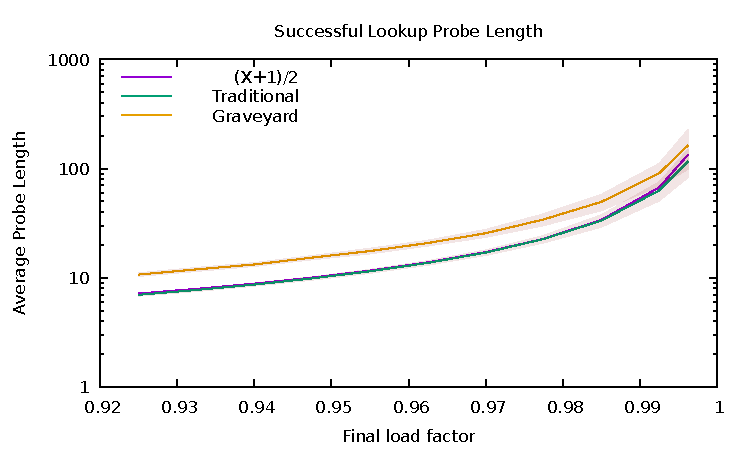
\includegraphics[width=75mm]{experiments/increasing-load-found}  &
  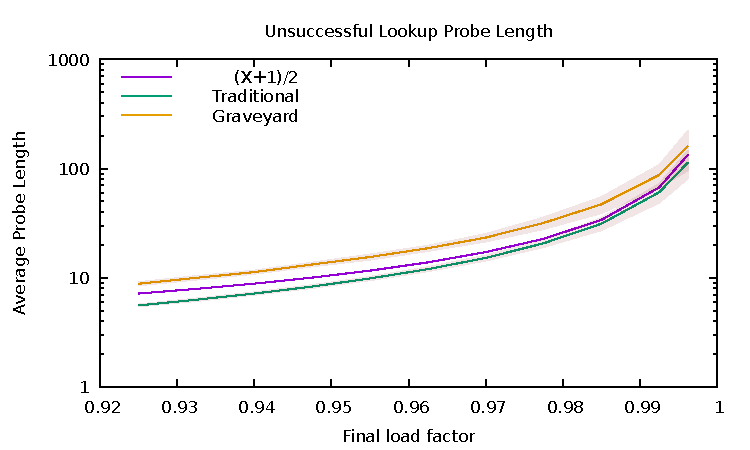
\includegraphics[width=75mm]{experiments/increasing-load-notfound}  \\
  \begin{minipage}{75mm}
    % TODO Get this font right.
    \footnotesize (a) Successful Lookup, comparing Graveyard,
    Traditional (both with 95\% confidence intervals shown, shaded),
    and Knuth's prediction $(X+1)/2$.
  \end{minipage}
  &
  \begin{minipage}{75mm}
    % TODO Get this font right.
    \footnotesize (a) Unsuccessful Lookup, comparing Graveyard,
    Traditional, and Knuth's prediction $(X+1)/2$.
  \end{minipage}
 
  \\
  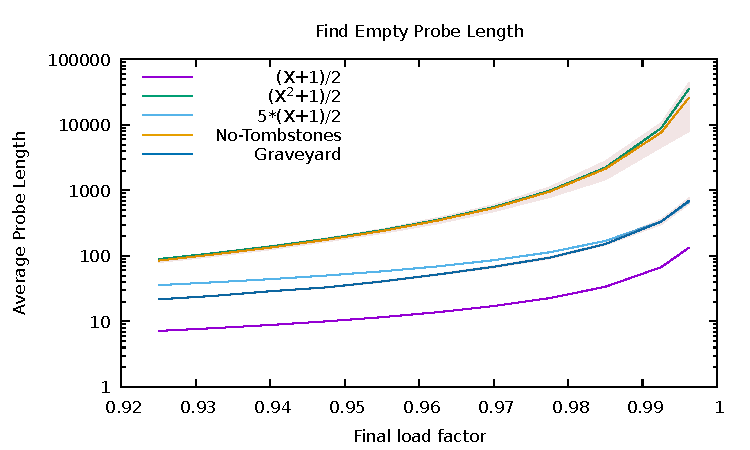
\includegraphics[width=75mm]{experiments/increasing-load-findempty} &
  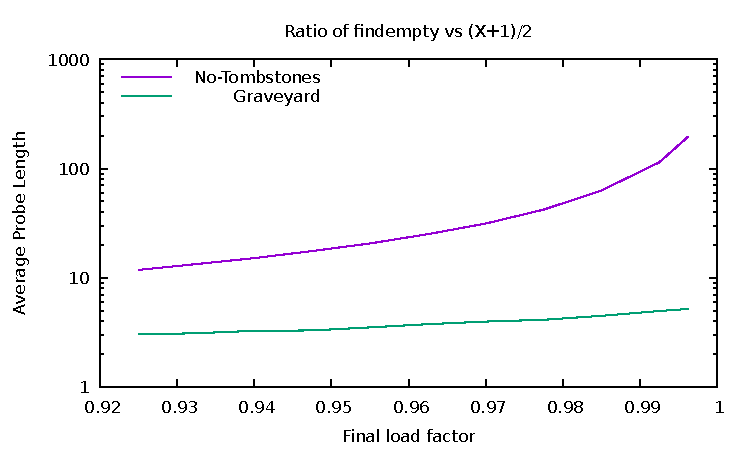
\includegraphics[width=75mm]{experiments/increasing-load-findempty-ratio}  \\
  \begin{minipage}{75mm}
    % TODO Get this font right.
    \footnotesize (a) Average probe length to find an empty slot for
    Graveyard, Traditional, and showing Knuth's $(X+1)/2$ prediction
    for lookup and $(X+1)/2$ prediction for insert.
  \end{minipage}
  &
  \begin{minipage}{75mm}
    % TODO Get this font right.
    \footnotesize (a) How much worse is find-empty than Knuth's
    lookup?  Graveyard is a small factor (staying near 4 even for very
    high load factors, traditional grows quickly.
  \end{minipage}
 
  \end{tabular}
\end{center}
\caption{How query-optimized graveyard hashing scales as the load factor increases.}
\figlabel{probelengths}
\end{figure}

\section{Experiment 2}

The second experiment is to vary the number of tombstones that are put
in during rehashing.  The theory \cite{BenderKuKu22} says that if you
are going to insert $k$ values between rehashing, then you should put
in $ck$ tombstones for some constant greater than one.  Increasing $c$
makes lookups slower, since during rehash fewer slots were available,
and the values get spread around further as though the load factor was
higher.  (TODO: Write the expression down.)  But it makes subsequent
inserts faster, since there are more empty slots in which to insert.
(We cannot raise $c$ so high that all the free slots are used).

For our first guess we set $c=2$.  This experiment shows the tradeoff
as we vary $c$, called the \textit{graveyard factor}.

\figref{varytombstones} shows the tradeofff.  We have heard that for
most hash tables, lookups are the dominant operation (perhaps
accounting for 60\% to 90\% of the operations), so the choice of
$c=2$, where lookups are about 3 times faster than inserts looks
pretty good.  If we lower $c$ to, say $5/3$, then the ratio is about
$6$ and the choice is good only when lookups are 90\% or more of the
operations.  (TODO: Is there a visualization of this tradeoff?)  If we
raise $c$ to, say $3$ then lookups become more expensive than inserts.
We conclude that $2$ is about right.

\begin{figure}
  \begin{center}
  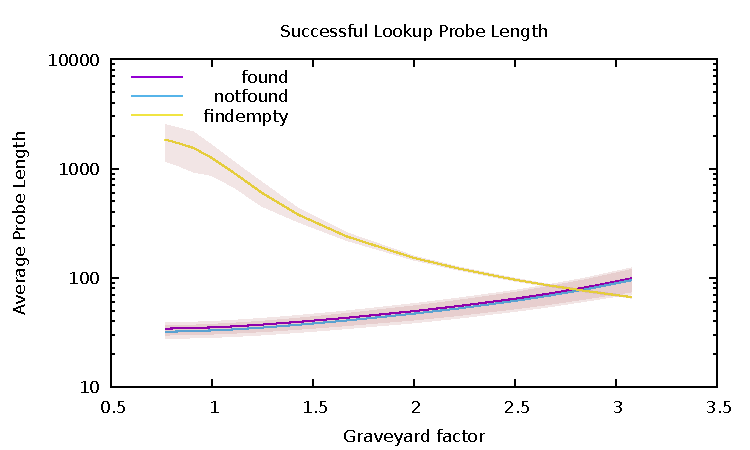
\includegraphics[width=75mm]{experiments/vary-tombstones}
  \end{center}
  \caption{Increasing the graveyard factor makes lookups slower and
    inserts faster, in a table that is filled to 98\% full, rehashed
    with tombstones, and then 0.5\% more keys are added.  The table is
    10,000,000 elements.}
  \figlabel{varytombstones}
\end{figure}

\section{Experiment 3: Ordered-Linear-Probing with Tombstones Spike}

\figref{olpspike} shows ordered linear probing with tombstones sees a
spike in the average insertion cost as the table reaches the high load
factor, but then the average insertion cost quickly falls as
tombstones are inserted.  In this figure, $X=200$, so Knuth's formula
predicts an insertion cost of $(X^2+1)/2=20000$, whereas the actual
peak is about 8700, and the search cost at the end of the insertion
phase $(X+1)/2 = 100$ and the actual number is around 70.  These
numbers have high variations and we ran only one experiment.
\todo{multiple experiments with confidence intervals.}

\begin{figure}
\begin{center}
\begin{tabular}{cc}
  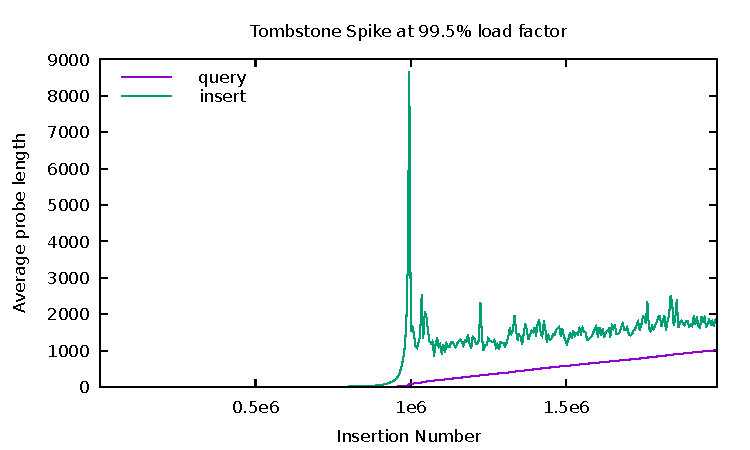
\includegraphics[width=75mm]{experiments/spike-1000000-0.995000} &
  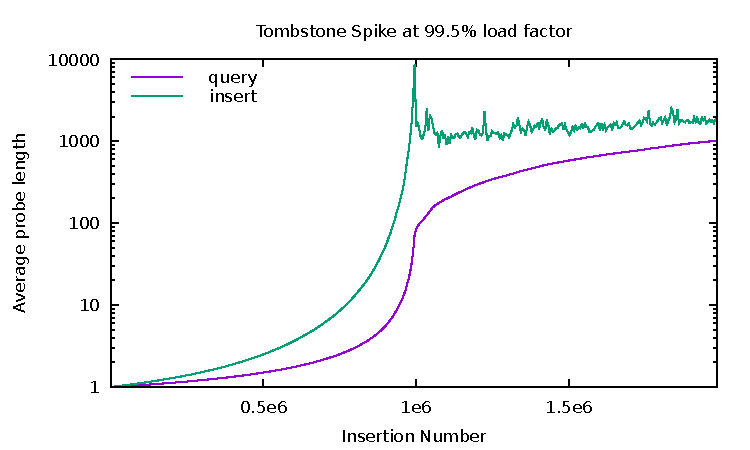
\includegraphics[width=75mm]{experiments/spike-1000000-0.995000-log} \\
  (a) On a linear scale & (b) On a log scale.
\end{tabular}
\end{center}
\caption{Ordered-linear-probing with tombstones on an insertion-only
  workload (left half) followed by a hovering workload (right half).
  The query cost stays low during the insertion workload, and starts
  rising during the hovering workload.  The insertion cost jumps very
  high near the end of the insertion phase, and drops dramatically
  during the hovering phase.}
\figlabel{olpspike}
\end{figure}

\section{Experiment 4: Traditional Spike}

How well does the search distance work?

\section{Experiment 5: Compare our library to others}

\figref{libraries} shows some microbenchmarks for our library,
compared to Abseil~\cite{Abseil17}\footnote{Abseil commit
\texttt{81927248} Mar 21, 2023.}, F14~\cite{BronsonSh19}\footnote{F14
commit \texttt{22b89282} Jan 30, 2023}, and Libcuckoo~\cite{LiAnKa14,
  GoyalFaLi23}\footnote{Libcuckoo commit \texttt{e1d74917} Jan 1,
2023.  Note that Libcuckoo provides a \texttt{map}, but does not
provide a \texttt{set}, and all our benchmarks are on \texttt{set}.
So LibCuckoo has larger value objects than the other experiments, and
our measurement of LibCuckoo's memory doesn't include the extra space
for the mapped value.}.

Libcuckoo is slower on all operations than the other tables.  It's not
too surprising that insertions are slow with cuckoo hashing, but the
lookups are slow too.  It turns out that Libcuckoo does not use vector
instructions, which probably is the reason lookups are slow.
Furthermore comparing Libcuckoo to Graveyard, F14, or Abseil is not an
apples-to-apples comparison since Libcuckoo offers concurrent accesses
using hardware transactional memory (which seems to be a dead
technology), and provides no reference stability (whereas the
convention adopted by F14 and Abseil is that references remain stable
unless the table is rehashed, and they provide a way to reason about
when the table will be rehashed.)

Google is the fastest except for successful loookups, where facebook
is the fastest.  Graveyard is a little slower, probably because of its
higher load factor.  \todo{State the load factors used by graveyard.}

\todo{Memory footprint and high-water marks.}

\begin{figure}
  \begin{center}
    \begin{tabular}{cc}
    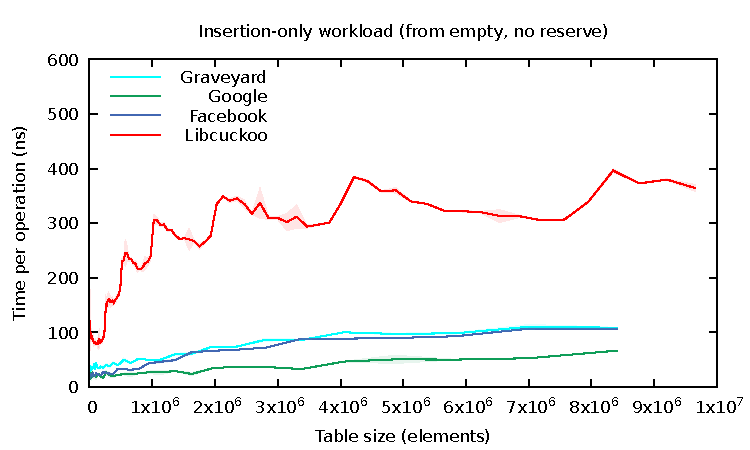
\includegraphics[width=75mm]{experiments/library-insertion} &
    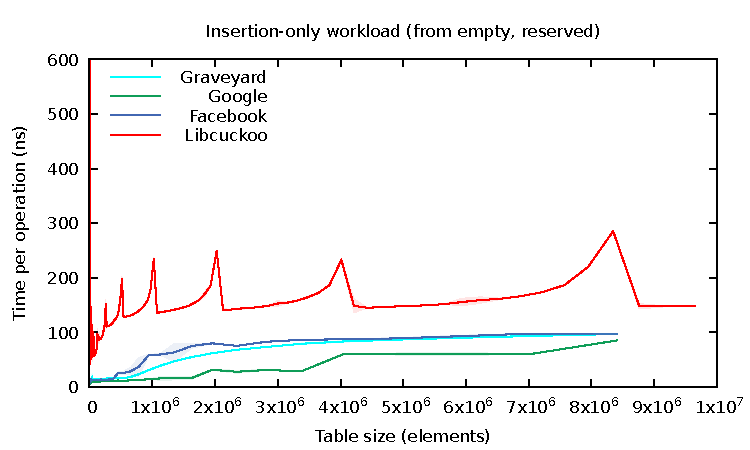
\includegraphics[width=75mm]{experiments/library-reserved-insertion} \\
    (a) Insertion of $n$ elements from empty without \texttt{reserve()}. &
    (b) Insertion of $n$ from empty with \texttt{reserve(n)}. \\
    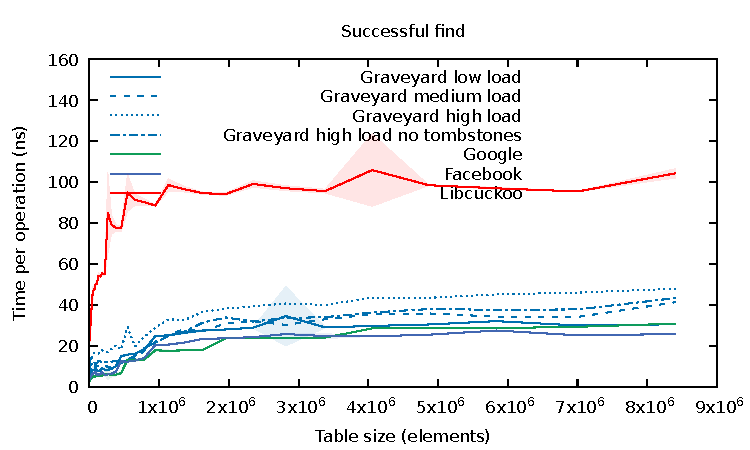
\includegraphics[width=75mm]{experiments/library-found} &
    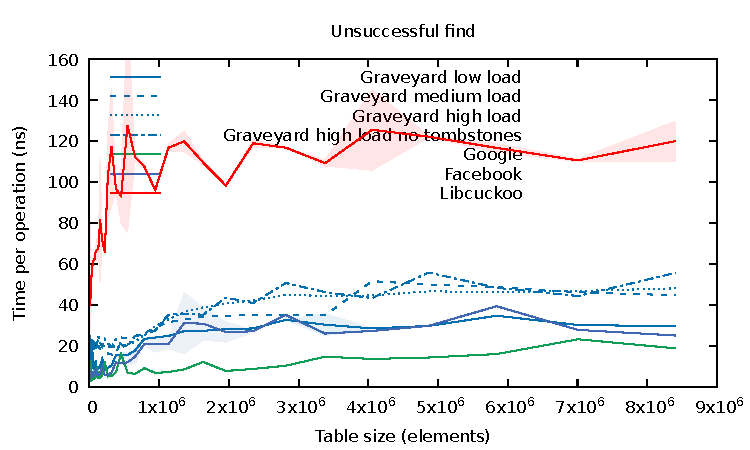
\includegraphics[width=75mm]{experiments/library-notfound} \\
    (c) Cost of successful lookup in a table of size $n$. &
    (d) Cost of unsuccessful lookup in a table of size $n$. \\
    \end{tabular}
  \end{center}
\caption{Comparison of the speed of Graveyard vs.~Google (Abseil)
  vs.~Facebook (F14) vs.~LibCuckoo.  The X axis is the table size, and
  the Y axis is the time-per-operation for the entire construction.
  Lower is better.  The shaded region shows a 95\% confidence interval
  (actually, two standard deviations).}
\figlabel{libraries}
\end{figure}

\section{Experiment}

How much does the hash function cost?


\bibliographystyle{plainurl}
\bibliography{hashing}

\end{document}
